%% LyX 2.3.6 created this file.  For more info, see http://www.lyx.org/.
%% Do not edit unless you really know what you are doing.


\documentclass[10pt]{article}
\usepackage{helvet}
\usepackage{caption}
\usepackage{float}
\usepackage{xcolor}
\usepackage[framemethod=TikZ]{mdframed}
\renewcommand{\familydefault}{\sfdefault}
\usepackage[T1]{fontenc}
\usepackage[utf8]{inputenc}
\usepackage[a4paper]{geometry}
\geometry{verbose,tmargin=2cm,bmargin=4cm,lmargin=2cm,rmargin=2cm}
\usepackage{fancyhdr}
\pagestyle{fancy}
\setlength{\parskip}{6pt}
\setlength{\parindent}{0pt}
\usepackage{tcolorbox}
\usepackage{amsmath}
\usepackage{amsthm}
\usepackage{amssymb}
\usepackage{todonotes}
\usepackage{graphicx}
\usepackage[backend=bibtex,maxbibnames=99]{biblatex}
\addbibresource{main.bib}

\floatstyle{plaintop}
\newfloat{listing}{htbp}{lop}
\floatname{listing}{Listing}

\definecolor{lightgray}{gray}{0.9} % Defines the color 'lightgray' with a specific shade.

\newmdenv[
  linecolor=lightgray,
  backgroundcolor=white,
  outerlinewidth=1pt,
  roundcorner=2pt,
  innertopmargin=10pt,
  innerbottommargin=10pt,
  innerrightmargin=10pt,
  innerleftmargin=10pt
]{greyborder}


\makeatletter

\DeclareMathOperator*{\argmin}{arg\,min}

%%%%%%%%%%%%%%%%%%%%%%%%%%%%%% LyX specific LaTeX commands.
%% A simple dot to overcome graphicx limitations
\newcommand{\lyxdot}{.}

%%%%%%%%%%%%%%%%%%%%%%%%%%%%%% User specified LaTeX commands.
\usepackage{tcolorbox}
\usepackage{amsthm}
\usepackage{lastpage}
\usepackage{fancyhdr}
\usepackage{accents}
\usepackage{titlesec}
\usepackage{marginnote}
% \titleformat{\section}[block]{\normalfont\bfseries}{}{0em}{}


\usepackage{enumitem}
\usepackage{comment}
% \setlist{nolistsep}

\usepackage{tcolorbox}
\definecolor{light-blue}{cmyk}{0.24, 0.12, 0.0, 0.04, 1.00}
% \titlespacing\section{0pt}{0pt}{0pt}
% \titlespacing\subsection{0pt}{0pt}{0pt}
% \titlespacing\subsubsection{0pt}{0pt}{0pt}

\setlength{\headheight}{40pt}

\makeatother

\title{Week 2 Optimisation for Machine Learning}
\author{Neimhin Robinson Gunning, 16321701}
\date{\today}

\begin{document}
\maketitle
\lhead{Neimhin Robinson Gunning} \rhead{CS7CS4 Week 2 Assignment}

\section{Part (a)}
\subsection{Part (a) (i)}
% [ ] TODO: Using sympy obtain an expression for the derivative dy/dx. Show all the steps that you used to obtain the expression.
To represent the expression $x^4$ using sympy we first create a symbol object for $x$ (line 1 in Listing~\ref{fig:ai-code}), and then raise it to the fourth power using standard python arithmetic notation. The \texttt{**} operation is overloaded such that \texttt{x**4} yields an object representing the expression $x^4$. If we assume $y(x)=x^4$ then the derivative $dy/dx$ is found with \texttt{(x**4).diff()}. Running the code we find this derivative to be $4x^3$.

\begin{listing}
  \begin{center}
    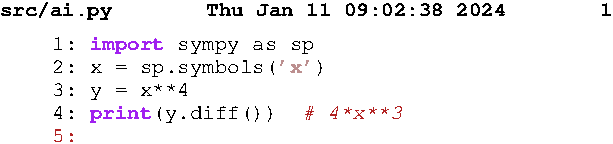
\includegraphics[width=0.45\textwidth]{fig/ai-code.pdf}
  \end{center}
  \caption{Source code to find the derivative of $x^4$ using sympy. The result is $4x^3$.}\label{fig:ai-code}
\end{listing}

\subsection{Part (a) (ii)}
% [ ] TODO: For a range of values of x calculate the derivative value using the expression from
% (i). Also calculate the derivative value estimated using a finite difference with
% perturbation δ = 0.01 on x. Plot these values on the same plot and compare.
% Show the code that you used to calculate the finite difference estimate.
\begin{listing}
  \begin{center}
    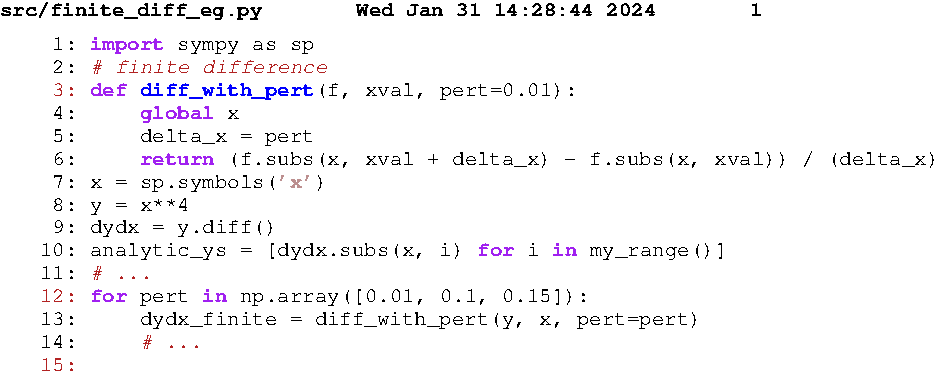
\includegraphics[width=0.45\textwidth]{fig/finite_diff_eg.pdf}
  \end{center}
  \caption{Ellided source code to estimate the derivative of $x^4$ using the finite difference method. The function \texttt{diff\_with\_pert} can be used to estimate the derivative of an arbitrary function of $x$. The full script is in the appendix and named \texttt{src/aii.py}.}\label{fig:ai-code}
  \label{listing:finite-diff}
\end{listing}

\subsection{Part (a) (iii)}
% [ ] TODO: For a range of values of x calculate the derivative value using the expression from
% (i). Also calculate the derivative value estimated using a finite difference with
% perturbation δ = 0.01 on x. Plot these values on the same plot and compare.
% Show the code that you used to calculate the finite difference estimate.
The accuracy of the finite difference approximation of the derivative is greater for smaller values of $\delta$. The reason for this
is related to the definition of the derivative. The derivative
is defined as $$\lim_{\delta\rightarrow 0}\frac{f(x+\delta)-f(x)}{x+\delta-x}$$, i.e. the derivative is the function approached by this expression as $\delta$ approaches 0. As we decrease $\delta$ and apply the finite difference method we are approaching the true derivative.
\begin{figure}
  \begin{center}
    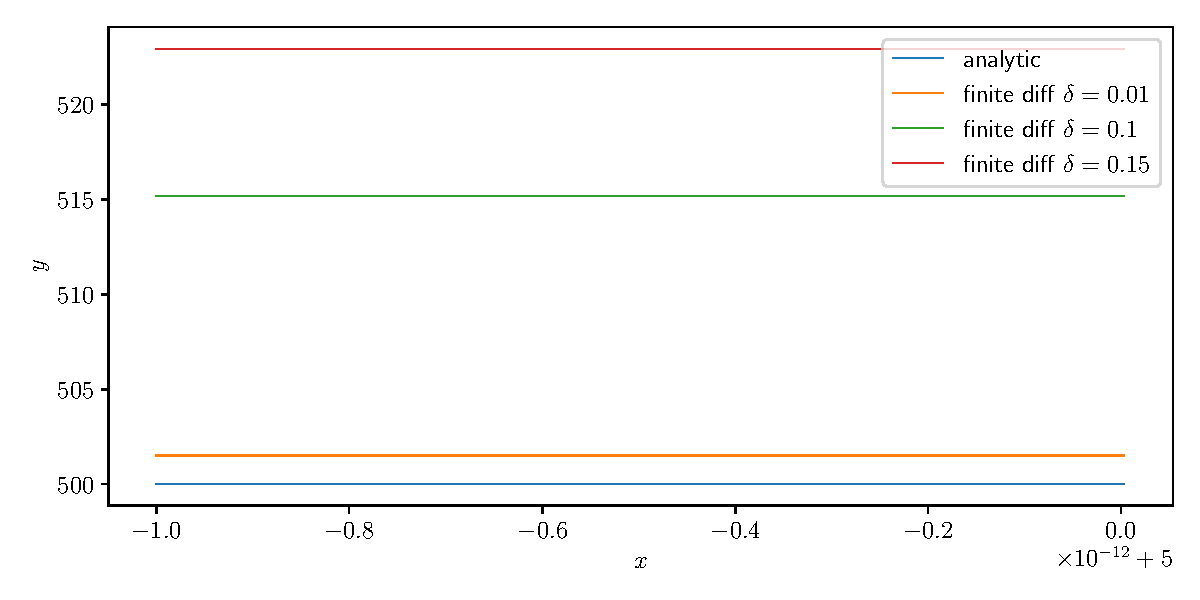
\includegraphics[width=0.95\textwidth]{fig/finite-diff.pdf}
  \end{center}
  \caption{A comparison of the analytic derivation of $dy/dx=4x^3$ and some approximations of $dy/dx$ using the finite difference method. The finite difference approximation was $\hat{\frac{dy}{dx}}(x)=\frac{(x + \delta)^4 - x^4}{\delta}$.}\label{fig:finite-diff-perterbations}
\end{figure}


\section{(b)}
\subsection{(b) (i)}
% [x] TODO: Write a short python programme that implements gradient descent with a fixed step size α. Explain your code.
Listing \ref{listing:gradient-descent} shows ellided source code for a python class that can be used to run gradient descent.
Ellided functions allow for specification of the function to be optimized, the convergence condition, the max number of iterations etc.
Line 13 calculates the gradient at the current value, and line 14 updates the value based on the gradient and step size. The convergence condition is a function of $x_n$ and $x_{n-1}$. Examples of this class in use are in the appendix, e.g. in \texttt{src/bi.py}, in which the gradient function is computed with \texttt{sympy}.

\begin{listing}
  \begin{center}
    \includegraphics[width=0.7\textwidth]{tmp/gradient_descent_listing.pdf}
  \end{center}
  \caption{Ellided source code a python class that implements gradient descent with a fixed step size.}\label{fig:ai-code}
  \label{listing:gradient-descent}
\end{listing}


\subsection{(b) (ii)}
% [ ] TODO: With initial value x = 1 and step sizes α = 0.1 run your gradient descent
% programme with the function y = x4 . Plot how x and y(x) vary with each
% gradient descent iteration. Discuss.

In Figure \ref{fig:gradient-descent-bi} is a plot of gradient descent on $x^4$ with $x_0=1$ and $\alpha=0.1$.
We see that updates to $|\hat x|$ and $y(\hat x)$ are initially large but quickly become tiny.
Because $x^4$ is very flat around the minimum (see subplot (c)) we have a very small gradient, and thus very small step sizes,
so the algorithm updates extremely slowly towards $\hat x=0$, but cannot reach it in a finite number of iterations.

\begin{figure}
  \begin{center}
    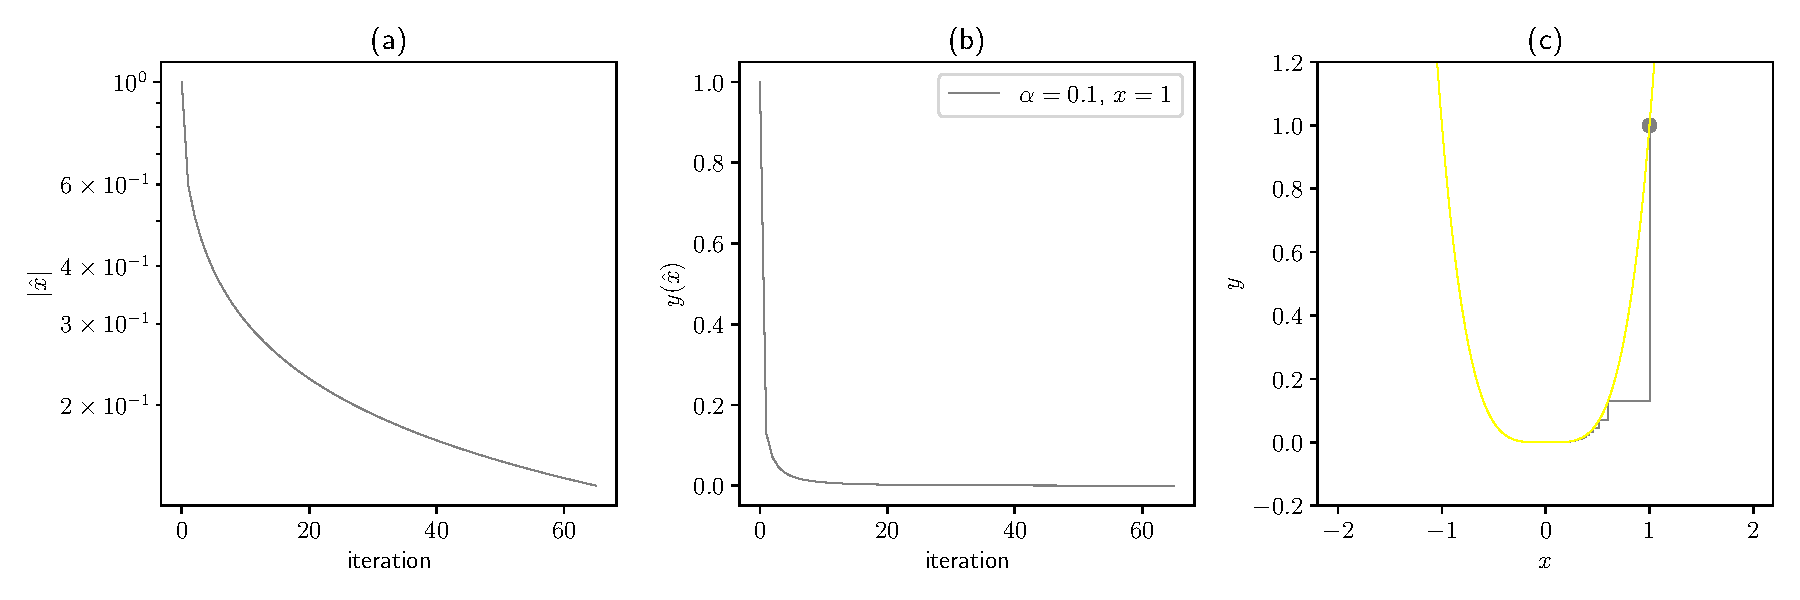
\includegraphics[width=0.95\textwidth]{fig/gradient-descent-bi.pdf}
  \end{center}
  \caption{Running gradient descent on $x^4$ with initial value $x_0=1$ and step size $\alpha=0.1$. 
  The yellow line in subplot (c) is $x^4$.}\label{fig:gradient-descent-bi}
\end{figure}

% [ ] TODO: Now repeat (ii) for a range of initial values for x and step sizes α. Be sure to
% choose a large enough range of step sizes that you see a variety of behaviours
% (including non-convergence)
% How does the choice of alpha affect the convergence time? Why?
In Figure \ref{fig:gradient-descent-b1} several runs of gradient descent on
$x^4$ are visualized. Subplot (a) shows $|\hat{x}|$ for each iteration, which is the distance of the estimate $\hat{x}$ from
the optimal value, $x=0$. With initial value $x=1$ and step size $\alpha=0.1$ we see that the steps are initially large, i.e. moving quickly to the optimum, but on successive iterations the steps slow down dramatically. In subplot (b) we see the value of $y(\hat{x})$ on each iteration.
  
The convergence criterion for gradient descent adopted here
is when $|\alpha\Delta x|<0.001$ or $x$ is $\pm\infty$\footnote{Meaning the floating point values \texttt{math.inf} or \texttt{-math.inf}}.
For the function $x^4$ we can see from Table \ref{tab:alpha-start-convergence} that the final guess, i.e. the estimate of $\argmin x^4$ is
most accurate and converges fastest with larger values of $\alpha$, \textbf{unless} $\alpha$ is too large and the iterations of gradient descent degenerate, i.e. subsequent iterations give worse or unchanged estimates.
The reason for this is that the gradient of $x^4$ is tiny as $x$ approaches the minimum. So, a smaller value of $\alpha$ means the convergence condition, $|\alpha\Delta x|<0.001$, can be met with a higher value of $\Delta x$, but in the case of $x^4$, $\Delta x$ is higher when $x$ is further from the optimal value 0. This is why the final guess
is worse for smaller values of $\alpha$, but why does a smaller
$\alpha$ lead to slower convergence time?

Since $\alpha$ is constant for a single run of gradient descent, the convergence condition depends on $\Delta x$, namely we need $|\Delta x|<0.001/\alpha$. A larger $\alpha$ entails a larger step, but there
are two factors at play here:
\begin{enumerate}
  \item A larger step size may entail a smaller $\Delta x$ on the subsequent iteration.
  \item A larger step size moves us away from meeting the convergence condition.
\end{enumerate}
It turns out for $x^4$ that the first of these factors is more important, in cases where gradient descent is converging. Thus larger $\alpha$ results in faster convergence (for $x^4$).

\begin{figure}
  \begin{center}
    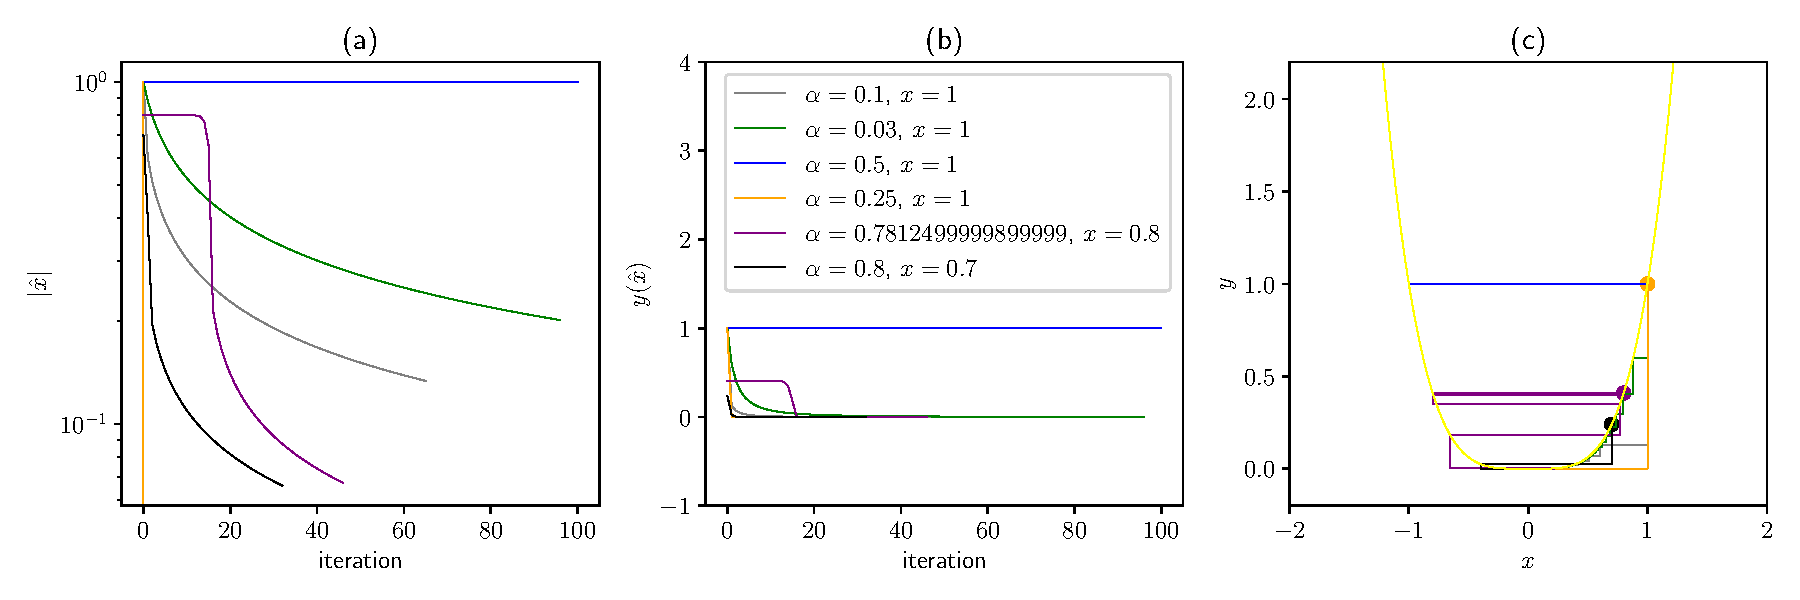
\includegraphics[width=0.95\textwidth]{fig/gradient-descent-b1.pdf}
  \end{center}
  \caption{Various runs of gradient descent on $x^4$. One run, where $\alpha=0.5$ and $x_0=1$, is stuck in a 2-step loop, flipping $\hat x$ back and forth between 1 and -1.
  The yellow line in subplot (c) is $x^4$.}\label{fig:gradient-descent-b1}
\end{figure}

\begin{table}
  \caption{Various runs of gradient descent on $x^4$ with different outcomes. The maximum number of iterations was set to 100, and the convergence threshold to $0.001$. Some of the $\alpha$ values were purposefully selected to lie near the margin of non-convergence, which can be calculated with $\alpha_m=\frac{2x_0}{4x_0^3}$. So rows 8 and 9 use $\alpha_m\pm\epsilon$.}
  \label{tab:alpha-start-convergence}
  \begin{center}
    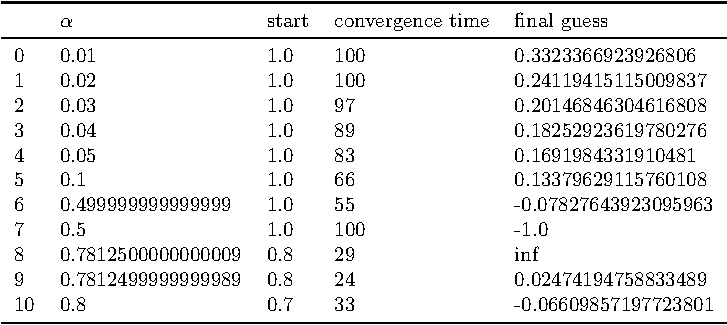
\includegraphics[width=0.95\textwidth]{fig/gradient-descent-b2.csv.pdf}
  \end{center}
\end{table}

\section{(c)}
\subsection{(c) (i) Optimising $\gamma x^2$}
% [ ] TODO How does changing \gamma affect the convergence of your gradient descent program? Why?
Firstly, note that if $\gamma$ is negative, then $\gamma x^2$ and $\gamma |x|$ have no
minimum, and thus gradient descent will behave weirdly. For instance, in my implementation,
with enough iterations it will actually finish with \texttt{math.inf}, which is reasonable.
If $\gamma=0$ then gradient descent terminates immediately, and any value for $x$ minimizes $\gamma x^2=0x^2$.
Increasing $\gamma$ increases the magnitude of the gradient, resulting in larger steps,
but the convergence time and accuracy will then depend on the initial value.

Let $d_0=|x_0-\argmin_x\gamma x^2|$ be the initial distance to the optimal value of $x$.
Let's assume $x_0$ is `far' from $$\argmin_x\gamma x^2$$, i.e. $d_0$ is large,
meaning gradient descent will at first take several steps in the same direction.
Increasing $\gamma$ to $\gamma'$, i.e. $\gamma'>\gamma$, results in a larger gradient $2\gamma' x'_0 > 2\gamma x_0$
meaning the first step is larger.
If after the first iteration the distance has improved, $d_1 < d_0$ then gradient descent will converge, if not it will diverge.
Let's assume we are in a converging condition.
While the second gradient $2\gamma' x'_1$ is not necessarily larger than $2\gamma x_1$, the updated $x'_1$ is now closer to the minimum than
$x_1$. The result of these dynamics is that with a larger $\gamma'$ there is
a fewer number iterations until the first `overshoot'.

For certain values this means that convergence time is smaller for the larger $\gamma'$ than for $\gamma$.

\subsection{(c) (ii) Optimising $\gamma |x|$}
% [ ] TODO How does changing \gamma affect the convergence of your gradient descent program? Why?

\begin{figure}
  \begin{center}
    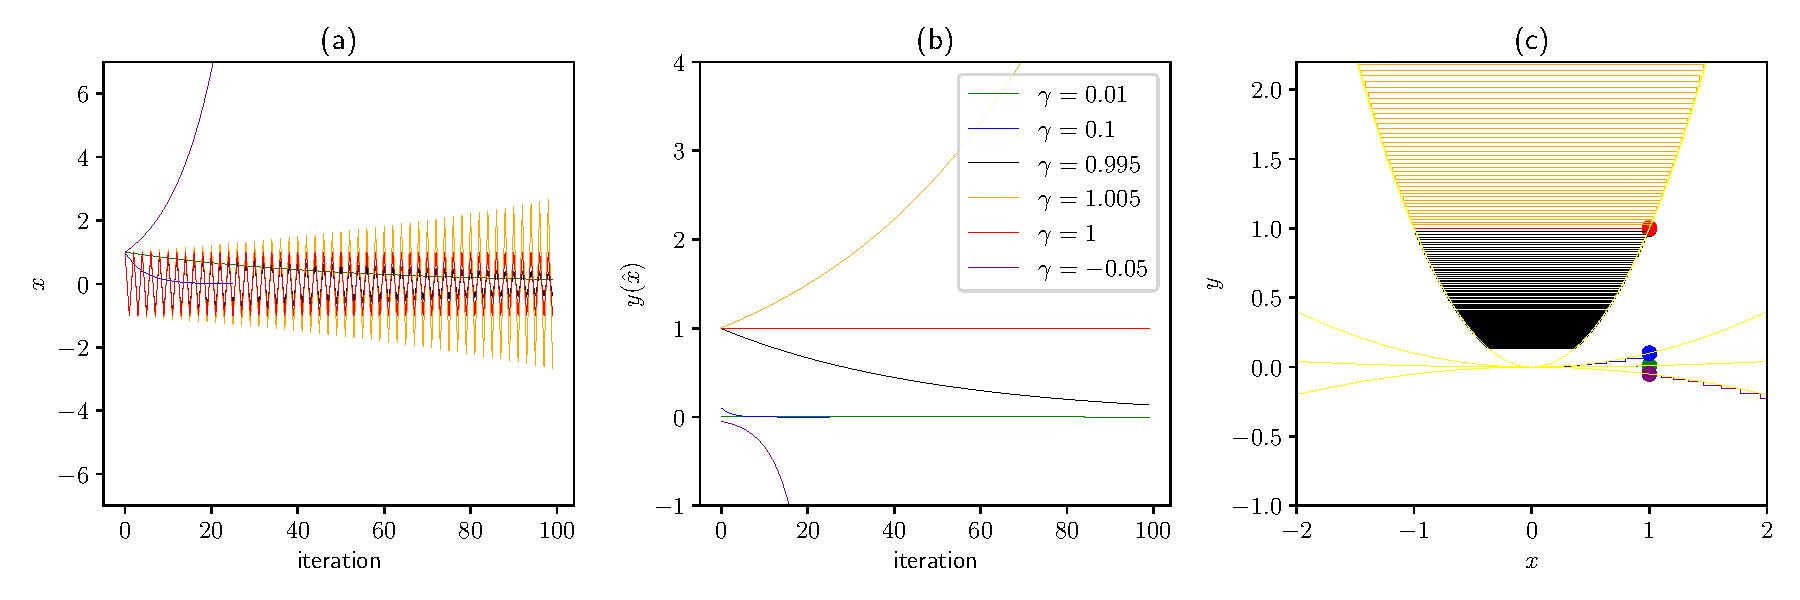
\includegraphics[width=0.95\textwidth]{fig/gradient-descent-ci.pdf}
  \end{center}
  \caption{
    Various runs of gradient descent on $\gamma x^2$.
    Subplot (a) shows the estimate of $x$ for each iteration.
    The yellow lines in subplot (c) are plots of the various $\gamma x^2$ functions.
  }\label{fig:gradient-descent-ci}
\end{figure}

\bigskip{}
\printbibliography
\end{document}
